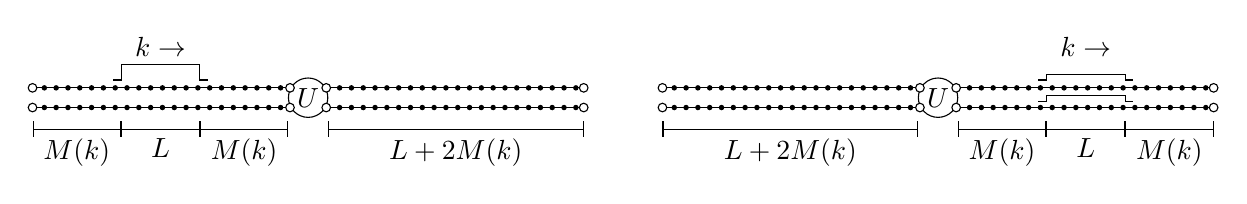
\begin{tikzpicture}[
  scale = 0.5,
  unitary/.style={circle,draw=black,fill=white,
    inner sep=0pt,minimum size=5mm},
  verts/.style={circle,fill=black,inner sep=.7pt,minimum size=0},
  attach/.style={circle,fill=white,draw=black,inner sep=1.1pt,minimum size=0pt}]
  \draw (-2,0.25) to (12,0.25);
  \draw (-2,-0.25) to (12,-0.25);

  \foreach \x in {-2,-1.7,...,12}{
  \foreach \y in {-.25,.25}{
    \node at (\x,\y) [verts] {};
  }}

  \node (1) at (5,0) [unitary] {$U$};

  \draw[xshift=-1cm] (1.05,.45) to (1.25,.45) to (1.25,.85) to (3.25,.85) 
           to (3.25,.45) to (3.45,.45);

  \node (momentum) at (1.25,1.3) [] {$k\rightarrow$};

  \draw[|-|] (-2,-.8)   to node[below] {$M(k)$} (0.25,-.8);
  \draw[|-|] (0.25,-.8) to node[below] {$L$}   (2.25,-.8);
  \draw[|-|] (2.25,-.8) to node[below] {$M(k)$} (4.5,-.8); 

  \draw[|-|] (5.5,-.8) to node[below] {$L + 2M(k)$} (12,-.8);

  \foreach \x in {-2, 12, 4.54, 5.46}{
  \foreach \y in {-.25, .25}{  
    \node at (\x,\y) [attach]{};
  }}

\begin{scope}[xshift=4cm]
  \draw (10,0.25) to (24,0.25);
  \draw (10,-0.25) to (24,-0.25);
  
  \foreach \x in {10,10.3,...,24}{
  \foreach \y in {-.25,.25}{
    \node at (\x,\y) [verts] {};
  }}
  
  \node (2) at (17,0) [unitary] {$U$};
 
  \draw[xshift=1cm] (18.55,.45) to (18.75,.45) to (18.75,.6)
     to (20.75,.6) to (20.75,.45) to (20.95,.45);

  \draw[xshift=1cm] (18.55,-.1) to (18.75,-.1) to (18.75,.05)
     to (20.75,.05) to (20.75,-.1) to (20.95,-.1);

  \node (momentum2) at (20.75,1.3) [] {$k\rightarrow$};


  \draw[|-|] (10,-.8) to node[below] {$L+2M(k)$} (16.5,-.8);
  \draw[|-|] (17.5,-.8) to node[below] {$M(k)$} (19.75,-.8);
  \draw[|-|] (19.75,-.8) to node[below] {$L$} (21.75,-.8);
  \draw[|-|] (21.75,-.8) to node[below] {$M(k)$} (24,-.8);
  
  \foreach \x in {10, 24, 16.54, 17.46}{
  \foreach \y in {-.25, .25}{  
    \node at (\x,\y) [attach]{};
  }}
\end{scope}
\end{tikzpicture}